%!xelatex = 'xelatex --halt-on-error %O %S'

\documentclass{thuemp}
\usepackage{url}
\usepackage{lipsum}  % 生产假书乱文的包,实际使用时可去掉
\usepackage{hyperref}
\begin{document}

% 标题,作者
\emptitle{基于强化学习的无人机飞跃冰湖实验}
\empauthor{傅信燊,秦华谦,向航,张祖烨(拼音顺序)}{古博老师}

% 奇数页页眉 % 请在这里写出第一作者以及论文题目
\fancyhead[CO]{{\footnotesize 傅信燊,秦华谦,向航,张祖烨: 基于强化学习的无人机飞跃冰湖实验}}


%%%%%%%%%%%%%%%%%%%%%%%%%%%%%%%%%%%%%%%%%%%%%%%%%%%%%%%%%%%%%%%%
% 关键词 摘要 首页脚注
%%%%%%%%关键词
\Keyword{强化学习,冰湖问题,无人机}
\twocolumn[
\begin{@twocolumnfalse}
\maketitle

%%%%%%%%摘要
\begin{empAbstract}
  本次机器人综合实验的主题是无人机飞越冰湖。为了解决传统无人机避障算法中需要构建离线三维地图的问题,实验采用了基于马尔可夫决策过程的Qlearning、Sarsa和Double DQN(DDQN)算法。在Deterministic模式和Stochastic模式下的4x4及8x8地图上进行了相应的强化学习(RL)模型训练。通过性能比较,成功地在实机演示中控制无人机安全地飞越冰湖。
\end{empAbstract}

%%%%%%%%英文标题、作者、摘要、关键词
\emptitleEn{UAV flying over a frozen lake experiment based on reinforcement learning}
\empauthorEn{Fu Xinshen, Qin Huaqian, Xiang Hang, Zhang Zuyi}{Prof. Gu Bo}
\KeywordEn{Reinforcement learning, glacial lake problems, UAV}

\begin{empAbstractEn}
  The theme of this comprehensive robot experiment was the use of drones to fly over an ice lake. To address the issue of traditional drone obstacle avoidance algorithms requiring the construction of offline 3D maps, the experiment employed Qlearning, Sarsa, and Double DQN (DDQN) algorithms based on Markov Decision Processes. These algorithms were trained on corresponding Reinforcement Learning (RL) models on 4x4 and 8x8 maps under both Deterministic and Stochastic modes. Through performance comparisons, the experiment successfully demonstrated the control of drones flying over an ice lake in real machine demonstrations.
\end{empAbstractEn}

%%%%%%%%首页角注,依次为实验时间、报告时间、学号、email
\empfirstfoot{2023-11-27}{2023-11-30}{21312463 21312683 21312505 20354171}{qinhq5@mail2.sysu.edu.cn}
\end{@twocolumnfalse}
]
%%%%%%%%!首页角注可能与正文重叠,请通过调整正文中第一页的\enlargethispage{-3.3cm}位置手动校准正文底部位置:
%%%%%%%%%%%%%%%%%%%%%%%%%%%%%%%%%%%%%%%%%%%%%%%%%%%%%%%%%%%%%%%%
%  正文由此开始
\wuhao 
%  分栏开始

%=================================================================
\section{概~~述}
\enlargethispage{-3.3cm}

小型多旋翼无人机因其小巧灵活的特性,适宜在复杂环境中执行机动任务,因此在军用和民用领域得到了广泛应用。随着科技的进步,针对无人机的导航、指导和控制技术也获得了显著提升。然而,实时进行自主导航尤其在未知和结构不确定的三维环境中,尤其是在变化多端的光照条件下,仍然是一个极具挑战性的问题。这些环境中实现自主避障仍是一个迫切需要解决的问题。

\begin{figure}[H]
  \centering
  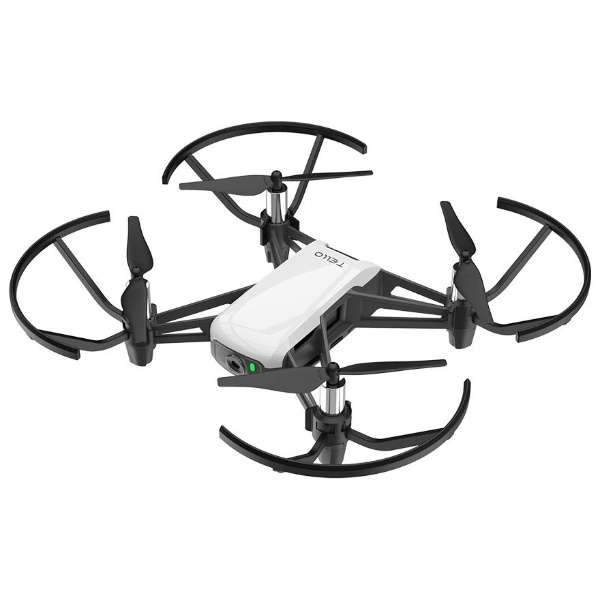
\includegraphics[width=0.8\linewidth]{./img/UAV.jpg}
  \caption{小型四旋翼无人机}
\end{figure}
传统的无人机避障算法依赖于构建离线三维地图,并在此基础上使用路径搜索算法来规划最优路径,这些路径以障碍物为约束。尽管一些避障算法避免了复杂的地图构建工作,它们仍需要手动调整大量参数,且在避障过程中无法利用经验进行自我迭代。随着机器学习的发展,研究人员开始将有监督学习应用于无人机避障,把避障任务视作一个基于监督学习的分类问题,但这需要对每个样本进行耗时的标注工作。

在无人机避障过程中,如何有效利用三维空间信息,避免繁琐的环境构建工作,简化算法模型,以及提升无人机的自主避障能力和效率,从而更安全、高效地到达指定目的地,仍是当前亟需解决的关键问题。

随着机器学习技术的进步,强化学习已经被科研人员应用于无人机控制领域。强化学习通过与外部环境的交互来优化行为,相比于传统机器学习方法,它具有以下优势:
  
\begin{enumerate}
  \item 在训练前,强化学习不需要对数据进行标注处理,这使得它能更有效地处理环境中的特殊情况;
  \item 强化学习可以将整个系统视为一个统一整体,从而实现端到端的输入输出。这使得系统的某些模块具有更强的鲁棒性;
  \item 相比其他机器学习方法,强化学习更容易学习一系列的行为。
\end{enumerate}
  
使用强化学习算法的优势在于它不依赖于传统非机器学习方法所需的离线地图,也不依赖于监督学习中所需的人工标注数据集。通过深度学习模型,强化学习学习输入数据与输出行为之间的映射关系,从而使智能体能够处理高维连续空间中的决策问题,并避免了复杂的离线地图构建工作。
  
基于这些优势,我们的研究小组通过查阅资料,对多种强化学习算法在冰湖环境下进行了仿真实验和性能对比。最终,我们选择了表现最佳的 Sarsa 算法,并成功应用于实际无人机飞越冰湖的演示中。
\begin{figure}[H]
  \centering
  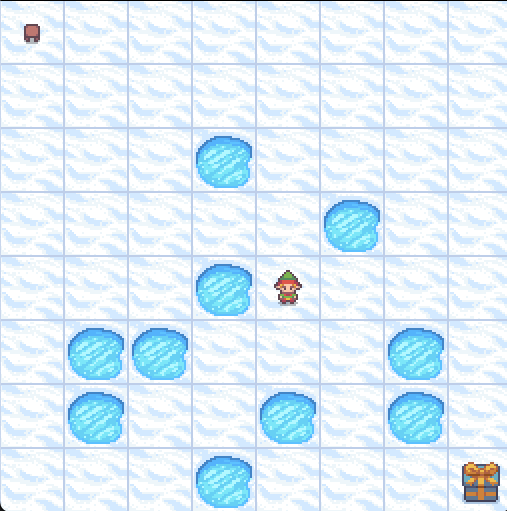
\includegraphics[width=0.8\linewidth]{./img/icelake1.png}
  \caption{冰湖实验环境}
\end{figure}



%======================================================
\section{算法介绍}
\subsection{强化学习(RL)}
强化学习(RL)是一种机器学习方法,它使得智能体(agent)通过与环境的交互来学习如何达到一个或多个目标。
这种学习方式与人类或动物学习经验的过程有相似之处,即通过试错的方式逐渐适应环境并实现目标。

强化学习过程中的一些关键概念如下:
\begin{itemize}
  \item 智能体(Agent): 在RL中,智能体是进行决策的实体,它选择执行哪些行为(actions)。
  \item 环境(Environment): 智能体所处并与之交互的外部世界或系统。
  \item 状态(State): 环境在任何特定时间点的状态。智能体的决策通常基于环境的当前状态。
  \item 行为(Action): 智能体在特定状态下可以执行的操作。
  \item 回报(Reward): 智能体执行特定行为后,环境提供的即时反馈。这是评价智能体行为好坏的标准。
  \item 策略(Policy): 策略是从状态到行为的映射。它定义了智能体在特定状态下应该采取的行为。
\end{itemize}

agent通过与环境交互来进行学习。这是一个以目标为导向的学
习过程,agent从其行为的结果中学习。agent可以根据最好的结果探索不同行为,也可以
利用获得了良好回报的先前行为。如果agent探索不同
的行为(action),则很有可能agent将获得较差的回
报,因为所有的行为并不都是最佳的。如果agent仅利
用已知的最佳行为,那么错过最佳行为(action)的可
能性也很大。因此,需要选择合适的算法在这两者间取
得平衡。
一个典型 RL 算法的步骤如下:
\begin{enumerate}
  \item 首先,agent通过执行行为与环境进行交互;
  \item agent执行行为并从一种状态移动到另一种状态;
  \item 然后agent将根据其执行的行为获得回报;
  \item 根据回报,agent将知道行为是好的还是坏的;
  \item 如果 action 是好的,也就是说,如果agent得到了积极的reward,那么agent将更喜欢执行该action,否则agent将尝试执行导致积极reward的其他action。
\end{enumerate}
强化学习作为一种机器学习方法,其独特性在于它强调在不确定和复杂的环境中通过交互学习,
使得它在实时决策和自适应控制方面尤为有效。随着算法和计算能力的不断发展,
强化学习未来在更多领域的应用前景看好。\\
\vbox{}
%============================================================
\subsection{Q-Learning}
在强化学习中,智能体(agent)通过与环境的交互来学习如何最大化累积奖励。
Q-Learning是强化学习中的一种重要算法,其名称来源于它使用的一个核心组件——Q表。\cite{csdn-ql}
\begin{figure}[H]
  \centering
  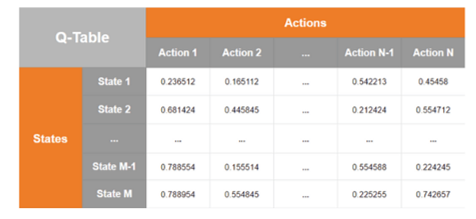
\includegraphics[width=0.8\linewidth]{./img/q-table.png}
  \caption{Q表示例}
\end{figure}

Q表是一种数据结构,用于存储和更新每个状态-动作对的值(Q值),
$Q$即为$Q(s, a)$, ,就是在某一时刻的s状态下$s(s\in S)$
采取动作$a(a\in A)$动作能够获得收益的期望,环
境会根据agent的动作反馈相应的回报reward r,所
以算法的主要思想是$Q$表随着状态、动作而更新,当
$Q$表更新不再发生改变时,就可以根据环境选择对应
最大的值所对应的动作,从而采取动作,进行与环境交
互。

$Q$表的更新是通过一种称为时间差分学习的方法进行的。
在每一步中,智能体根据当前的$Q$表选择一个行为,执行该行为后,它接收到一个奖励和新的状态信息。
然后,使用这个新信息来更新$Q$表中当前状态和行为的$Q$值。

Q-learning 算法的更新准则如下式所示:
$$Q[S,A]=(1-\alpha)*Q[S,A]+\alpha*(R+\gamma*\max Q[S_next;])$$

其中,$\alpha$是学习率,决定了新信息覆盖旧信息的速度;R是即时奖励;
$\gamma$是折扣因子,用于平衡即时奖励和未来奖励;$S_next$是新状态;

构建$Q$表算法步骤:

Step 1: 给定参数$\gamma$和reward矩阵$R$

Step 2: 令$Q:=0$

Step 3: For each episode:

3.1 随机选择一个初始的状态$s$

3.2 若末达到目标状态,则执行以下几步:
\begin{enumerate}
  \item 在当前状态$s$的所有可能行为中选取一个行为$\alpha$
  \item 利用选定的行为$\alpha$,得到下一个状态$\tilde{s}$
  \item 按照算法更新公式计算$Q(s, a)$
  \item 令$s:=\widetilde{s}$
\end{enumerate}

在Q-Learning中,智能体的策略通常是一种贪婪策略,即在大多数情况下选择当前Q值最高的行为。然而,为了鼓励探索,通常会加入一定比例的随机行为选择,这称为$\epsilon$-贪婪策略。

Agent利用上述算法从经验中进行学习。每一个
episode相当于一个training session。在一个training session中,agent探索外界环境,并接收外界环境的
reward,直到达到目标状态。训练的目的是要强化agent
的“大脑”(用$Q$表示)。训练得越多,则$Q$被优化得更
好. 当矩阵$Q$被训练强化后,agent便很容易找到达到
目标状态的最快路径了。

利用训练好的矩阵$Q$,我们可以很容易地找出一条
从任意状态$s_0$出发达到目标状态的行为路径,具体步
骤如下:

1. 令当前状态$s := s_0$

2. 确定$a$,它满足$Q(s,a)=\max_{\tilde{a}}\{Q(s,\widetilde{a})\}.$

3. 令当前状态$s:=\widetilde{s}$($\tilde{s}$表示$a$对应的下一个状态)

4. 重复执行步2和步3直到$s$成为目标状态

当Q表中的值不再发生显著变化时,我们认为算法已经收敛。此时,Q表提供了在每个状态下采取每个可能行为的最优策略。

通过使用Q-Learning,智能体能够学习在各种不同的状态下采取何种行为以最大化总奖励。这种学习方法在处理复杂、未知或变化的环境中显示出了巨大的潜力,尤其是在那些难以用传统算法编程解决的问题上。\\
\vbox{}
%===================================================
\subsection{Srasa}
Sarsa\cite{amazon}这个名字来源于五个关键因子:S(State当前状态)、A(Action当前行动 
)、R(Reward即时奖励)、S(State下一时刻的状态)和A(Action下一时刻的行动)。

Sarsa算法的的决策部分与Q-learning相同,都是
通过$Q$表的形式进行决策,在$Q$表中挑选值较大的动
作值施加在环境中来换取奖惩,也就是根据计算出来的
$Q$值来作为选取动作的依据,两者不同的是行为更新准
则是有差异的。在Q-Learning中,智能体会选择它认为可能获得最大Q值的下一个行为,
即使这个行为并未实际执行。而在Sarsa算法中,智能体更新当前行为的Q值时,
使用的是实际执行的下一个行为的Q值。
(Sarsa不会去选取他估计出来的最大$Q$
估计值,而是直接选取估计出来的$Q$值)。
\begin{figure}[H]
  \centering
  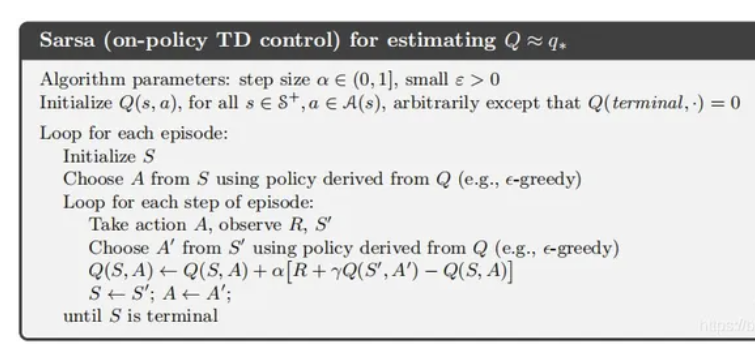
\includegraphics[width=0.8\linewidth]{./img/sarsa.png}
  \caption{Sarsa}
\end{figure}

Sarsa算法的更新准则如下式所示:
$$Q[S,A]=(1-\alpha)*Q[S,A]+\alpha*(R+\gamma*Q[S_{next},A_{next}])$$

其中,$S$和$A$分别代表当前状态和行为,$R$是获得的即时奖励,$\gamma$是折扣因子,
$S_{next}$和$A_{next}$分别是下一个状态和实际采取的下一个行为。

具体的改变就是在于:

$\max Q[S_next;]$变成了$Q[S_{next},A_{next}]$

Sarsa算法的这种更新方式使得其更加注重实际执行的路径,而不是仅仅追求理论上可能的最大回报。
这种方式使得Sarsa在某些情况下比Q-Learning更加稳健,因为它考虑到了实际的状态转移和行为选择。

在实际应用中,这意味着Sarsa算法倾向于选择一条相对安全的路径,尽可能避免陷阱和不确定性。
相比之下,Q-Learning更倾向于追求最快的路径,即使这条路径可能涉及更多的风险。
这种差异在某种程度上提高了Q-Learning的泛化能力,但也可能使其陷入局部最优解,
而忽视了更安全或可靠的解决方案。

总的来说,Sarsa算法通过其独特的更新准则,提供了一种更加注重实际执行路径的学习策略,
这在复杂和不确定的环境中可能更为有效。\\
\vbox{}
%=========================================
\subsection{DQN}
在Q-learning算法中,我们以矩阵的方式建立了一张存储每个状态下所有动作值的表格。
表格中的每一个动作价值表示在状态下选择动作,然后继续遵循某一策略预期能够得到的期望回报。
然而,这种用表格存储动作价值的做法只在环境的状态和动作都是离散的,并且空间都比较小的情况下适用。
当状态或者动作数量非常大的时候,这种做法就不适用了。
极端情况下,当状态或者动作连续的时候,就有无限个状态动作对,
我们更加无法使用这种表格形式来记录各个状态动作对的Q值。

对于这种情况,我们需要用函数拟合的方法来估计值,即将这个复杂的值表格视作数据,
使用一个参数化的函数来拟合这些数据。很显然,这种函数拟合的方法存在一定的精度损失,
因此被称为近似方法。DQN算法便可以用来解决连续状态下离散动作的问题。

由于神经网络具有强大的表达能力,因此我们可以用一个神经网络来表示函数Q。\cite{csdn-dqn}
在动作是离散(有限)的情况下,除了可以采取动作连续情况下的做法,
我们还可以只将状态输入到神经网络中,使其同时输出每一个动作Q的值。

假设神经网络用来拟合函数的参数是 ,即每一个状态下所有可能动作a的Q值我们都能表示为$Q_{\omega}(s, a)$。
我们将用于拟合函数函数的神经网络称为Q网络.

那么 Q 网络的损失函数是什么呢?我们先来回顾一下 Q-learning 的更新规则
$$Q[S,A]=(1-\alpha)*Q[S,A]+\alpha*(R+\gamma*\max Q[S_next;])$$

上述公式用时序差分(temporal difference,TD)学习目标$R+\gamma*\max Q[S_next;]$来增量式更新$Q[S,A]$,
也就是说要使和 TD 目标$R+\gamma*\max Q[S_next;]$靠近。
于是,对于一组数据,我们可以很自然地将 Q 网络的损失函数构造为均方误差的形式:
$$\omega^*=\arg\min_\omega\frac{1}{2N}\sum_{i=1}^N\left[Q_\omega\left(s_i,a_i\right)-\left(r_i+\gamma\max_{a'}Q_\omega\left(s_i',a'\right)\right)\right]^2$$

至此,我们就可以将Q-learning扩展到神经网络形式——深度Q网络(deep Q network,DQN)算法。
由于DQN是离线策略算法,因此我们在收集数据的时候可以使用一个$\epsilon$-贪婪策略来平衡探索与利用,
将收集到的数据存储起来,在后续的训练中使用。DQN中还有两个非常重要的模块——经验回放和目标网络,
它们能够帮助DQN取得稳定、出色的性能。

\textbf{经验回放(评估网络):}

在一般的有监督学习中,假设训练数据是独立同分布的,我们每次训练神经网络的时候从训练数据中随机采样一个
或若干个数据来进行梯度下降,随着学习的不断进行,每一个训练数据会被使用多次。
在原来的 Q-learning 算法中,每一个数据只会用来更新一次值。
为了更好地将 Q-learning 和深度神经网络结合,DQN 算法采用了经验回放(experience replay)方法,
具体做法为维护一个回放缓冲区,将每次从环境中采样得到的四元组数据(状态、动作、奖励、下一状态)
存储到回放缓冲区中,训练 Q 网络的时候再从回放缓冲区中随机采样若干数据来进行训练。
这么做可以起到以下两个作用。

(1)使样本满足独立假设。在MDP中交互采样得到的数据本身不满足独立假设,
因为这一时刻的状态和上一时刻的状态有关。非独立同分布的数据对训练神经网络有很大的影响,
会使神经网络拟合到最近训练的数据上。采用经验回放可以打破样本之间的相关性,让其满足独立假设。

(2)提高样本效率。每一个样本可以被使用多次,十分适合深度神经网络的梯度学习。

\textbf{目标网络:}

DQN 算法最终更新的目标是让$Q_{\omega}(s, a)$逼近$R+\gamma*\max Q[S_next;]$,由于 TD 误差目标本身就包含神经网络的输出,
因此在更新网络参数的同时目标也在不断地改变,这非常容易造成神经网络训练的不稳定性。
为了解决这一问题,DQN 便使用了目标网络(target network)的思想:
既然训练过程中 Q 网络的不断更新会导致目标不断发生改变,不如暂时先将 TD 目标中的 Q 网络固定住。
为了实现这一思想,我们需要利用两套 Q 网络。

(1)原来的训练网络$Q_{\omega}(s, a)$,用于计算原来的损失函数中$\frac12[Q_{\omega}\left(s,a\right)-\left(r+\gamma\max_{a^{\prime}}Q_{\omega^{-}}\left(s^{\prime},a^{\prime}\right)\right)]^{2}$
的项,并且使用正常梯度下降方法来进行更新。

(2)目标网络$Q_{\omega^{-}}(s,a)$,用于计算原先损失函数$\frac12[Q_{\omega}\left(s,a\right)-\left(r+\gamma\max_{a^{\prime}}Q_{\omega^{-}}\left(s^{\prime},a^{\prime}\right)\right)]^{2}$中的$(r+\gamma\max_{a^{\prime}}Q_{\omega^-}\left(s^{\prime},a^{\prime}\right))$项,
其中$\omega^{-}$表示目标网络中的参数。如果两套网络的参数随时保持一致,
则仍为原先不够稳定的算法。为了让更新目标更稳定,目标网络并不会每一步都更新。
具体而言,目标网络使用训练网络$Q_{\omega}(s, a)$的一套较旧的参数,训练网络在训练中的每一步都会更新,
而目标网络的参数每隔C步才会与训练网络同步一次,即$\omega^{-}\leftarrow\omega $。
这样做使得目标网络相对于训练网络更加稳定。

具体来讲,流程如下:
\begin{figure}[H]
  \centering
  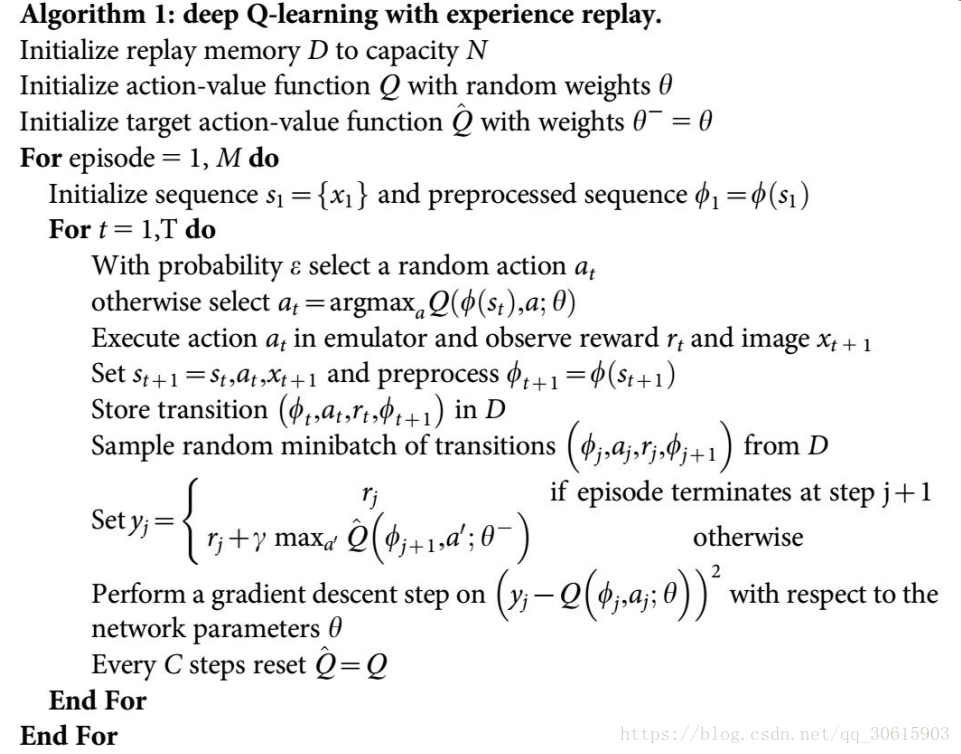
\includegraphics[width=1\linewidth]{./img/dqn.png}
  \caption{DQN算法流程}
\end{figure}

\subsection{Deterministic vs. stochastic}
当环境的下一个状态是由当前的状态以及 agent 要执行的 action 决定的,我们说它是Deterministic,
否则,说它是stochastic。在一个“完全可见的”,且“Deterministic”环境中,agent不需要担心不确定的东西。
比如在游戏中,agent是Deterministic,即使它不能预测其他玩家的行动。
而在现实中,形势太复杂,我们必须得看作是 stochastic,因为我们不可能知道所有不可见的因素。
如果一个环境不是完全可见的,或者不是 确定性的,我们说它是uncertain。
“stochastic”一般来说意味着后果的不确定性在概率上是可以量化的。
nondeterministic的环境是指action以它们可能的后果为特点,但是没有概率属性。
nondeterministic的环境通常用于描述衡量performace时agent达到action的所有可能的后果。

具体来讲,就是在随机环境中,状态转移和奖励不仅取决于当前状态和行为,还受到随机因素的影响。
这意味着对于相同的状态和行为,每次的结果(下一个状态和奖励)可能不同。
而在确定性环境中,给定当前状态和行为,下一个状态和奖励是完全确定的。\\
\vbox{}

\section{实验结果与分析}
\subsection{Deterministic模式}
在Deterministic模式下的实验中,我们分别对$Q-learning$和Sarsa两种强化学习算法进行了详细的比较和分析。
这两种算法都在处理相同的任务,并在相同条件下运行了300,000个Episodes。
通过绘制它们的收敛曲线,我们能够深入了解这两种算法的学习效率和行为特性。

通常每个Episode的奖励是检查收敛的最直接指标。如果奖励随时间变得稳定(不再有显著波动),
这意味着算法正在收敛。
因此使用滑动窗口平均($window_size=500$)的方法,在episode为300,000的情况下,
记录每个episode的全局rewards,将其视作模型的训练效果。作图如下:

\begin{figure}[H]
  \centering
  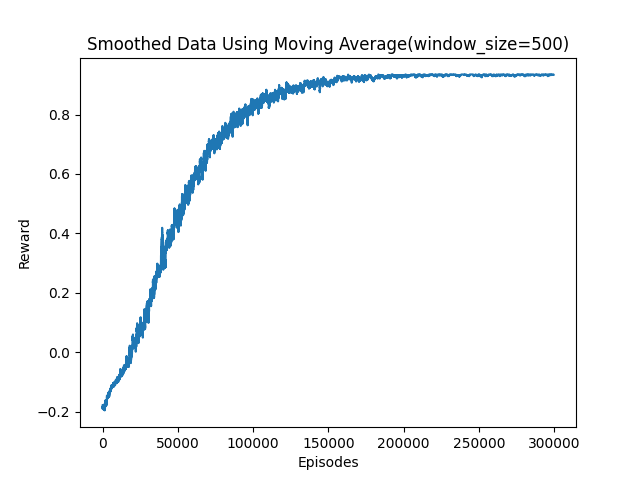
\includegraphics[width=1\linewidth]{./img/result/QL-rewards.png}
  \caption{$Q-learning$}
\end{figure}

\begin{figure}[H]
  \centering
  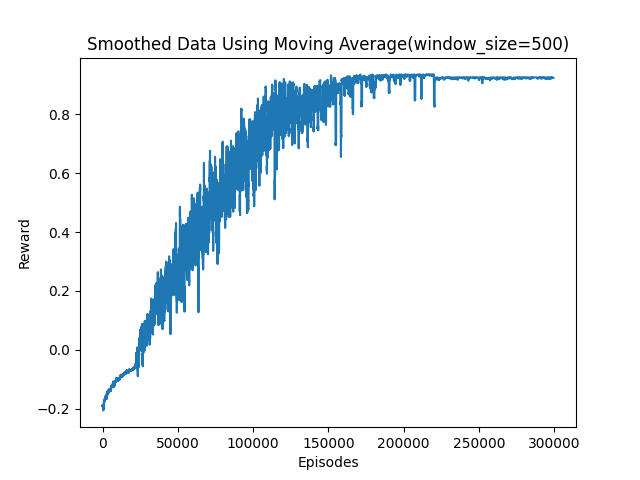
\includegraphics[width=1\linewidth]{./img/result/Sarsa-Rewards.png}
  \caption{Sarsa}
\end{figure}

收敛曲线表明,Q-learning和Sarsa算法都在大约150,000到200,000个Episodes之间达到了收敛状态。
这一现象表明,尽管两种算法在学习策略上有所不同,
它们在这个特定的任务中都能在相似的时间范围内学习到有效的策略。
然而,值得注意的是,多次实验并对比以后发现,Q-learning算法展现出了相对更快的收敛速度。
\begin{figure}[H]
  \centering
  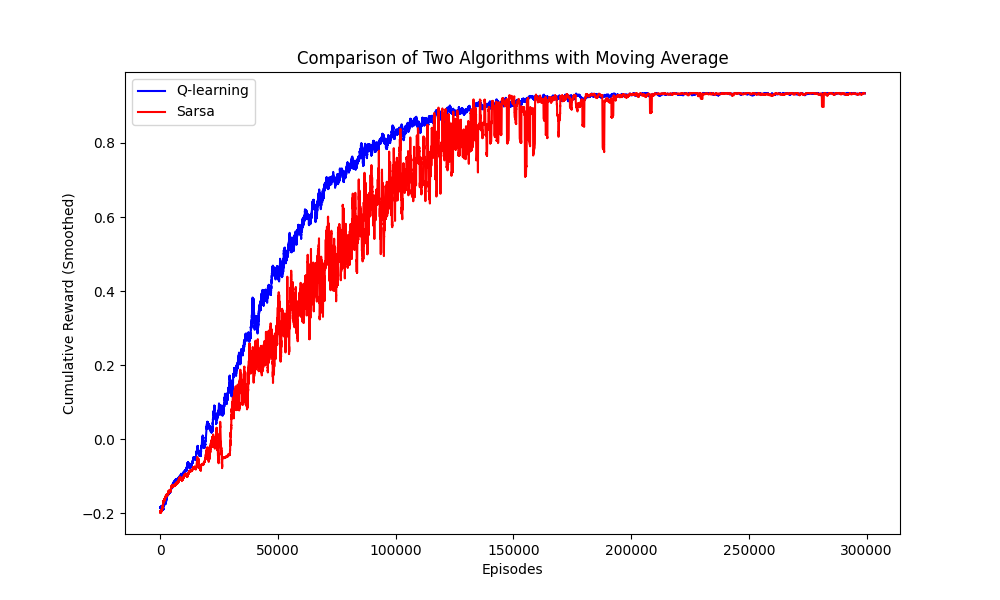
\includegraphics[width=1\linewidth]{./img/result/compare1.png}
  \caption{compare1}
\end{figure}
\begin{figure}[H]
  \centering
  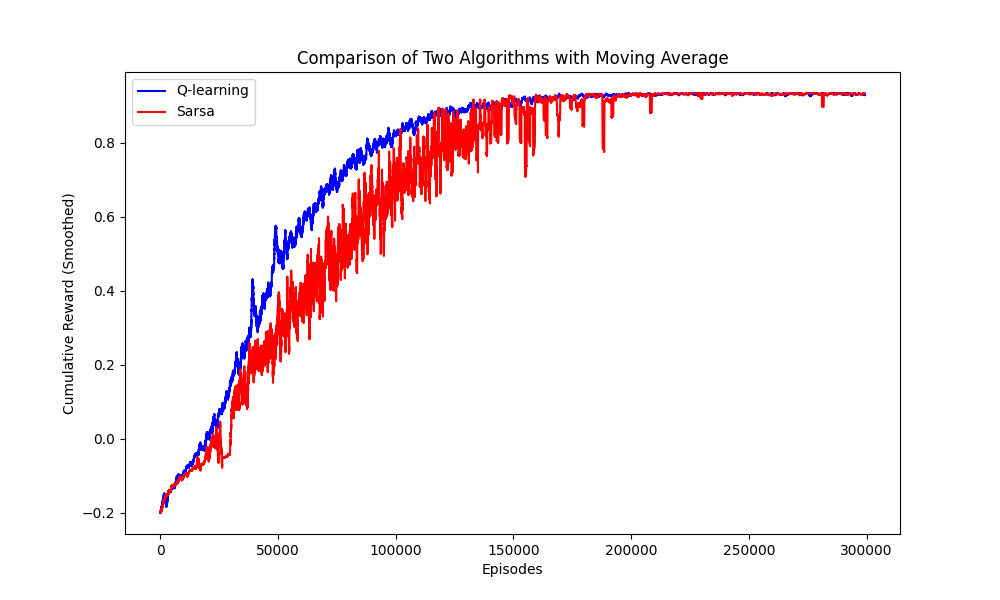
\includegraphics[width=1\linewidth]{./img/result/compare2.png}
  \caption{compare2}
\end{figure}
\begin{figure}[H]
  \centering
  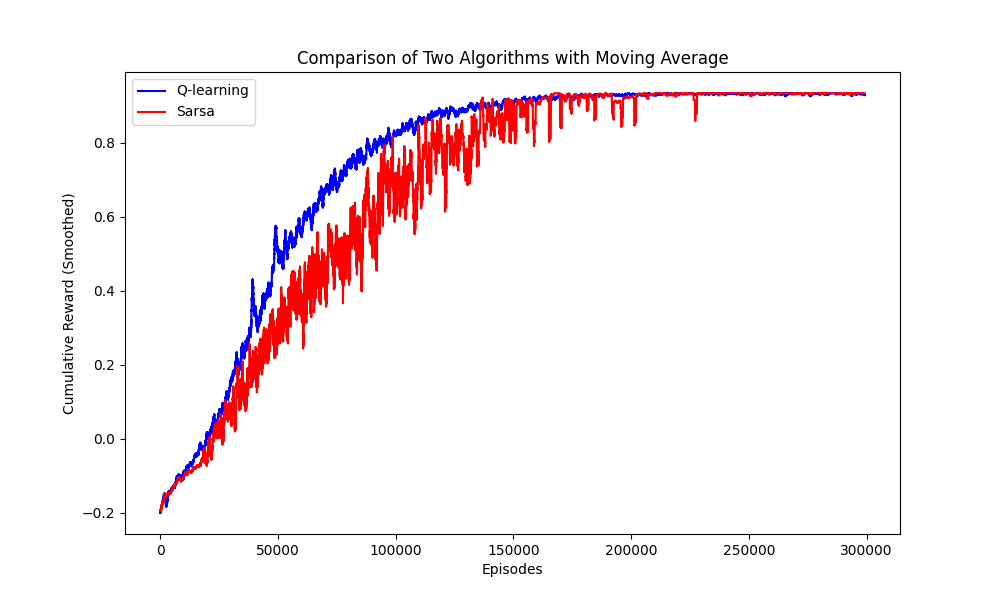
\includegraphics[width=1\linewidth]{./img/result/compare3.png}
  \caption{compare3}
\end{figure}

除了收敛速度外,我们还对两种算法的运行效率进行了对比。
运行时间的记录显示,在完成300,000个Episodes的任务中,Sarsa算法需要2分钟5秒,
而Q-learning算法仅需要1分钟40秒。这个时间差异虽然不是特别显著,但在大量Episodes累积下来的情况下,
这种效率的提升仍然是值得关注的。Q-learning算法更短的运行时间表明它在处理这类任务时可能更为高效。
这可能与其在更新价值估计时更为直接和积极的策略有关。

总体来看,在Deterministic模式下,Q-learning算法在收敛速度和运行效率上均表现出一定的优势。
这些发现对于选择和优化强化学习算法在特定任务和环境下的应用提供了重要的参考依据。\\
\vbox{}

\subsection{Stochastic模式}
在Stochastic(随机)模式下,对Q-learning和Sarsa两种强化学习算法进行了类似的实验和比较分析。
与Deterministic(确定性)模式相比,Stochastic模式下的环境为算法带来了新的挑战。
在这种模式下,我们也绘制了两种算法的收敛曲线进行观察。
\begin{figure}[H]
  \centering
  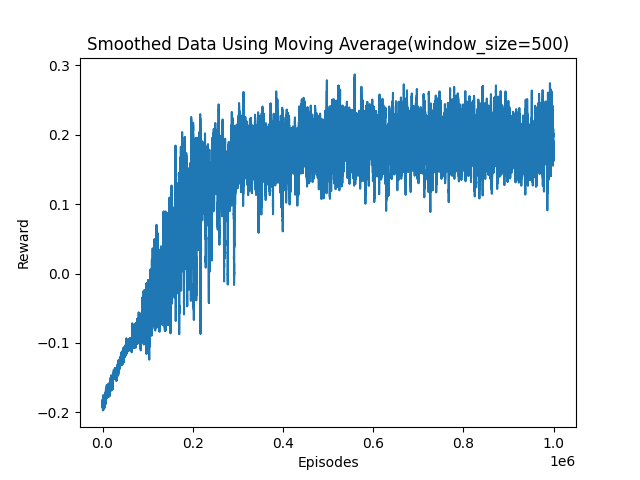
\includegraphics[width=1\linewidth]{./img/result/s/qls.png}
  \caption{Q-learning with Stochastic}
\end{figure}
\begin{figure}[H]
  \centering
  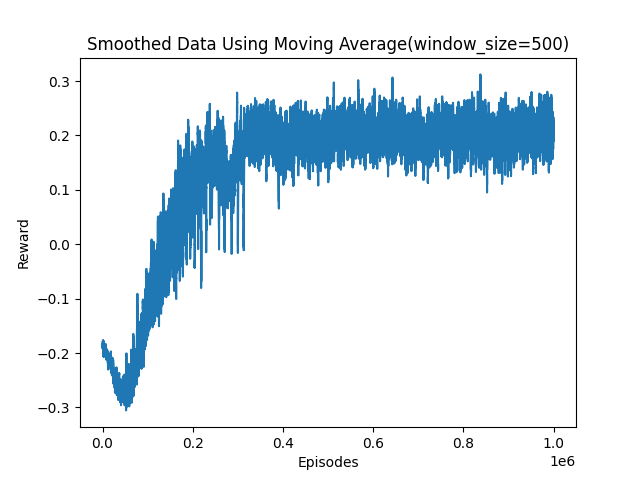
\includegraphics[width=1\linewidth]{./img/result/s/ss.png}
  \caption{Sarsa with Stochastic}
\end{figure}

不同于Deterministic模式,我们发现在Stochastic模式下,两种算法在收敛过程中表现出更大的振荡,
尤其是Q-learning算法。这种振荡表明了较差的稳定性,尤其是在算法的后期阶段。
在Stochastic模式中,代理执行动作后,环境的状态转移涉及到一定的随机性。
这意味着状态的转换不仅取决于代理的行动,还受到环境因素的影响,比如风力或冰面打滑等。
这与Deterministic模式形成鲜明对比,在后者中,环境状态的转换完全由代理的行动决定。
\begin{figure}[H]
  \centering
  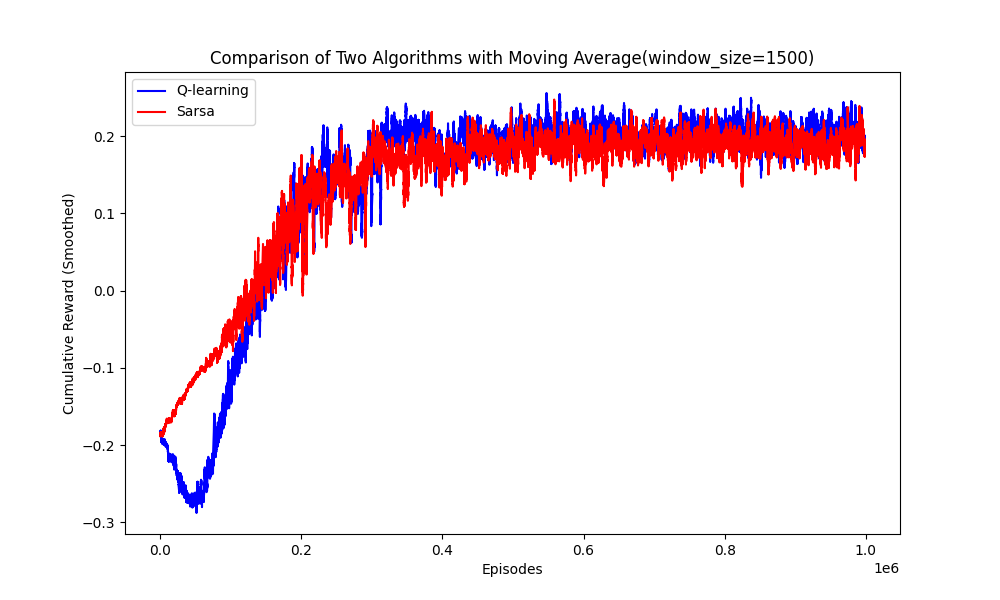
\includegraphics[width=1\linewidth]{./img/result/s/compare-s.png}
  \caption{Stochastic Mode Compare}
\end{figure}

由于Stochastic模式下状态转移的随机性,下一个状态$s_{t+1}$不仅仅与当前动作和当前状态$s_t$
有关,这增加了代理的学习难度。这种随机性使得算法难以稳定地学习一个稳定有效的策略,
因此,收敛变得更为困难。特别是对于Q-learning算法,这种挑战似乎更加显著,
因为其学习过程依赖于对未来奖励的估计,而在随机环境中这种估计更加困难和不稳定。

Sarsa算法,作为一种在策略内学习的方法,在面对这种随机性时,可能表现出相对更好的适应性,
因为其学习过程更加注重当前策略下的期望奖励,而不是像Q-learning那样依赖于最大化未来奖励的估计。

总体来说,在Stochastic模式下,环境的不确定性和随机性给强化学习算法的稳定性和收敛带来了额外的挑战,
这在Q-learning算法中表现得尤为明显。这些挑战需要通过改进算法或采用不同的策略来克服,
以便在这种更加复杂和不可预测的环境中实现有效的学习。\\
\vbox{}

\subsection{分析}
在比较Sarsa(一种on-policy学习算法)和Q-learning(一种off-policy学习算法)时,
我们可以看到两种方法在策略学习和探索方式上的根本差异。这些差异在Stochastic模式下的表现尤为明显,
因为环境的不确定性和随机性对学习过程产生了显著影响。

Sarsa作为一种on-policy算法,它的学习过程更加稳健和保守。
在每个Episode以及每个Step中,Sarsa都会执行epsilon-greedy探索策略,
这意味着即使在学习过程中,它也在一定程度上保留了探索新状态的可能性。
这种方法使得Sarsa能够更好地适应环境中的随机性,因为它的策略始终考虑了探索的元素。
然而,这种保守的学习方式也可能导致收敛速度相对较慢,特别是在环境较为复杂或存在较大随机性的情况下。

另一方面,Q-learning作为一种off-policy算法,更倾向于利用经验积累,寻找并学习到最优策略。
这种方法在收集和利用信息方面可能更高效,因为它专注于学习可能获得最大奖励的策略,
而不是当前策略下的期望奖励。这导致Q-learning在面对确定性环境时通常收敛更快。
然而,在Stochastic模式下,由于环境的不确定性和随机性,Q-learning可能表现出较大的波动性和不稳定性。
这是因为在随机环境中,对未来奖励的估计更加困难,
Q-learning的这种利用导向的学习策略可能导致它对环境变化的适应性不如Sarsa。

除了此次实验所展现的效果以外,在著名的悬崖行走曲线上,也能体现出来以上分析结果\cite{Ruoyu}————
q-learning方法是optimal的,但会有风险,sarsa方法是安全的,但学习的episode曲线也被拉长了。
\begin{figure}[H]
  \centering
  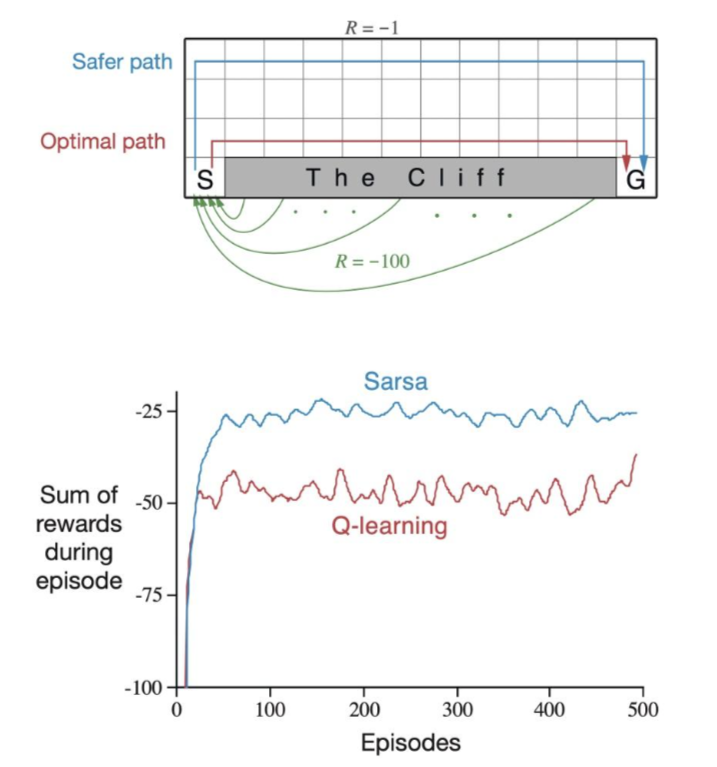
\includegraphics[width=1\linewidth]{./img/example.png}
  \caption{Example}
\end{figure}

综上所述,Sarsa的学习过程由于其在策略和动作上的同时考虑,可能更为保守,导致收敛时间较长,
但在随机环境中可能表现出更好的稳定性。而Q-learning由于其对最优策略的追求,可能在确定性环境中表现得更优,
但在面对随机环境时,其稳定性可能受到挑战。因此,在选择算法时,需要考虑到环境的特性以及算法的这些基本特征。\\
\vbox{}

\section{问题与解决}
\subsection{算法的效果展示与评估}
在强化学习性能评估中,通常有两种主要的方法:一是计算平均得分(即reward),
这涉及在agent执行一定步数后,记录其获得的所有奖励值并求其平均值;二是计算平均Q值,
即在测试性能前预先确定一定数量的状态-动作对,并在测试时计算这些确定状态-动作对的Q值的平均值。
在我们的实验中,选择了第一种方法,即求得分的方法。

然而,在绘制reward-epoch曲线时,我们发现了一个问题。
尽管这个曲线可以反映出随着训练轮数增加模型性能的变化趋势,但曲线的局部平稳性不佳,
容易出现“抖动”。这意味着相邻epoch的得分往往存在较大的差距。我们分析认为,这种现象的原因在于,
强化学习在每次迭代更新策略参数之后,相应的训练数据分布也发生变化。
这导致训练数据的分布往往与当前的策略分布存在一定差距,并且训练数据分布的更新也存在滞后性。
这可能使得算法在某些时刻对某些状态有较好的表现,而对另一些状态则表现较差。

为了解决这个问题,我们采用了滑动窗口平均的方法来平滑reward曲线。
这种方法通过计算在特定窗口内的平均值来减少短期波动的影响,从而使得长期趋势更加明显。
我们在曲线中应用了这种滑动窗口平均,这不仅使得曲线更加平滑,也更有助于观察和分析模型性能的真实趋势。

然而,由于实验条件的限制,以及强化学习训练本身耗费的时间巨大(Stochastic模式下训练一次用时30min),
我们在进行这项改进时适当减少了试验次数。
我们认为,即使在减少试验次数的情况下,
通过滑动窗口平均方法改善的reward-epoch曲线仍能有效地反映出模型性能的变化趋势,
并为我们提供更加稳定和可靠的性能评估。\\
\vbox{}

\section{实验总结}
通过本次实验任务,我们小组成员首次深入接触并认真研究了强化学习的相关知识,获得了宝贵的经验。
特别是将算法迁移到实机操作中的时候让我们学到很多。
这些经验教训表明,在强化学习的应用中,仅仅追求仿真环境中的SOTA性能是不够的。
算法的实际应用效果同样重要,特别是在处理实际物理环境中的不确定性和复杂性时。
为了提高算法在真实世界中的适用性和鲁棒性,我们需要更加关注算法与实际应用环境之间的紧密结合,
并在未来的工作中重视这一点。

目前,深度强化学习方法存在以下3个方面的局限性\cite{enderfga}:
\begin{enumerate}
  \item 深度强化学习理论支撑不够。谷歌的DeepMind团队于2015年在《自然》杂志上发表的文章虽然取得了较好的应用效果,但没有证明DQN的收敛性,并且到目前为止在DQN或其他深度强化学习方法的基础上的改进工作也没有很好地解决该问题。
  \item 样本采样率低。样本采样率低使得深度强化学习方法有时在实际应用中效果不佳。导致该问题的主要原因有两个:一是完成任务需要收集大量数据;二是训练过程中利用当前数据的有用信息效率低。
  \item 在连续动作空间中应用有限。目前主流的深度强化学习方法大多适用于离散动作空间,对于机器人的机械臂路径规划等连续动作空间的任务还处于初步研究阶段,理论支撑不够,因此应用十分有限。
\end{enumerate}

对于强化学习在应用中遇到的问题,我们认为未来的研究应着重关注以下几个方面,以期解决现有的困境和挑战:
\begin{enumerate}
  \item 设计有效的奖励函数:强化学习的核心在于通过最大化奖励值来寻求最优策略,而奖励函数的设计直接影响到所得策略的优劣。目前,奖励函数多由专家根据其专业知识设计,但随着路径规划领域应用环境的日益复杂化,传统的奖励函数设计方法可能不再适用。一些学者提出了元学习(Meta Learning)等新方法,旨在使智能体在面对环境或任务变化时,能从一系列合理的策略中不断优化其奖励函数。因此,设计有效且适应性强的奖励函数是未来研究的关键方向之一。
  \item 解决探索与利用的困境:在强化学习中,探索意味着不断尝试新的环境信息以获得更高的奖励值,防止陷入局部最优;利用则指依据已学习到的信息选择预期奖励最高的行为。探索与利用之间的平衡是强化学习中的一个核心问题。目前,E-greedy算法是常用的一种平衡方法,它让智能体以一定的概率随机探索或利用信息。虽然E-greedy算法简单易实现,但其随机探索效率低下,因此如何更高效地解决探索与利用的困境需要进一步研究。
  \item 研究强化学习与其他方法的结合:各种强化学习方法在应用于路径规划时都有其局限性。为了克服单一方法的不足,结合不同方法的优势可能是一个有效的策略。例如,传统的路径规划算法、图形学算法、智能仿生学算法与强化学习算法的结合,通过各自的长处相互补充,有望产生性能更佳的综合方法。
\end{enumerate}

当前,基于DQN的深度强化学习模型已相对成熟,策略梯度方法得到广泛应用,
同时元学习等领域的新算法也不断应用于深度强化学习。尽管如此,作为机器学习的新兴领域,
深度强化学习仍在不断发展之中,许多问题有待进一步探索和研究。我们团队也将持续学习相关知识,
努力在这一前沿领域进行深入探索。

%%=========================================================================

% \section*{写在最后}
% 在完成基于JMAG软件的三相永磁同步电机仿真分析的实验过程中,我经历了一段丰富而深刻的学习旅程,
% 对此我十分高兴并满怀感激之情。

% 首先,我要感谢我们的指导老师,您对三相永磁同步电机领域的深入讲解和专业指导,
% 使我得以将课堂上的理论知识与JMAG软件的实际操作相结合,从而深化了我的理解和掌握。
% 每次课堂上的精彩讲解都是如同指引航标,引导我在控制理论的海洋中航行。
% 这次实验不仅仅是对我所学知识的应用,更是一次宝贵的实践机会,
% 让我对永磁同步电机的工作原理有了更加深刻的认识。

% 同时,我也要特别感谢那些在网络上分享知识和经验的前辈和同行。
% 他们的文章和讨论为我提供了宝贵的参考资料,帮助我在遇到困难时找到了解决问题的思路。
% 特别是那些详细的JMAG操作指南
% 我也要特别感谢方桂安学长。虽然去年的作业要求与今年的不同,
% 但学长去年在博客上分享的报告\cite{JMAG}对我产生了深远的影响。在他的报告中,
% 我看到了深入浅出的解析和清晰的逻辑思维。您的报告让我深受启发,
% 也使我对电机的学习有了更深的认识和理解。我把您的博客网址和引用都标在了文末,
% 以表达我对您贡献的尊重和感谢。

% 这个实验过程不仅仅是对专业知识的应用,更是一次自我挑战和成长的历程。
% 在实验中,我不断地查阅资料,深入研究,理解和吸收了很多课堂上没有完全明白的知识点。
% 每一个小的发现和进步都让我感到无比的兴奋和满足。
% 然而,我也意识到我的水平还相当有限,还有很多东西我完全不了解或是一知半解,还有很多知识等待我去探索和学习。
% 我将把握住这次作业的契机,继续深入学习电机相关知识,争取能够了解很多,学会更多。

% 本着开源精神,我也将本次作业的所有模型和完成报告所用的\LaTeX 源文件全部托管在了GitHub仓库中,
% 以便老师和同学们进行浏览。

% 我诚挚地邀请每一位对此感兴趣的老师和同学,前往我的GitHub仓库查阅代码,
% 提出您的宝贵建议和批评。任何形式的反馈和建议,无论是关于代码的优化,
% 还是对于实验方法和结果的讨论,我都将热烈欢迎。我将珍惜所获得的一切知识和经验,
% 并继续在电机学的学习道路上不懈努力.


% GitHub repository URL: 

% \href{https://github.com/pbcn2/2023-HW-JMAG-three\_phase\_PMSM}{https://github.com/pbcn2/2023-HW-JMAG-three\_phase\_PMSM}

%%%%%%%%%%%%%%%%%%%%%%%%%%%%%%%%%%%%%%%%%%%%%%%%%%%%%%%%%%%%%%%%
%  参考文献
%%%%%%%%%%%%%%%%%%%%%%%%%%%%%%%%%%%%%%%%%%%%%%%%%%%%%%%%%%%%%%%%
%  参考文献按GB/T 7714-2015《文后参考文献著录规则》的要求著录. 
%  参考文献在正文中的引用方法:\cite{bib文件条目的第一行}

\renewcommand\refname{\heiti\wuhao\centerline{参考文献}\global\def\refname{参考文献}}
\vskip 12pt

\let\OLDthebibliography\thebibliography
\renewcommand\thebibliography[1]{
  \OLDthebibliography{#1}
  \setlength{\parskip}{0pt}
  \setlength{\itemsep}{0pt plus 0.3ex}
}

{
\renewcommand{\baselinestretch}{0.9}
\liuhao
\bibliographystyle{gbt7714-numerical}
\bibliography{./TempExample}
}



\end{document}

